\section{Simulation study}
\label{sec:simulation}

A simulation with a known ground truth answers questions that a short field study cannot: how much each source of information contributes, whether passive signals can be added safely, and how reliable the forecast is. The simulator (\texttt{web/src/sim/synth.ts}) and the evaluation (\texttt{web/scripts/simulate.ts}) call the same twin code as the website.

\subsection{Design}
\paragraph{Virtual participants.} Each virtual participant has a true sleepiness trajectory
\begin{equation}
  s^{*}(t) = \min\!\big(9, \max(1,\; p_{\phi}(t) + o + \gamma^{*} T(t) + \varepsilon(t))\big),
\end{equation}
where $p_{\phi}$ is the Three-Process Model prior with the person's circadian phase shifted by $\phi$, $o$ is a stable personal offset, $\gamma^{*}$ the person's time-on-task sensitivity and $\varepsilon$ a slow fluctuation (an Ornstein--Uhlenbeck process). Signals are generated from $s^{*}$ through person-specific mappings whose population distributions were taken from DROZY (Table~\ref{tab:population}): the PVT median reaction time is $r_0 + r_1(s^{*} - 3)$ plus noise, the mean blink duration is $b_0 + b_1(s^{*} - 3)$ plus noise, and PERCLOS is $\pi_0 + \pi_1 \max(0, s^{*} - 4)$ plus noise. KSS ratings are $s^{*}$ plus rating noise, rounded to integers and clipped to 1--9.

\paragraph{Cohorts.} Three disjoint cohorts with fixed random seeds were used. A \emph{training} cohort of 200 virtual people was used only to fit the population mappings, by ordinary least squares of KSS on each channel's features; the prior SDs of the weights were set to the between-person spread of per-person fits, with the per-person estimation noise removed by the method of moments. A \emph{tuning} cohort of 120 was used only to choose the webcam noise inflation $\kappa$, over a grid from 1 to 1280 and with the webcam switched off, at three check-ins. A \emph{test} cohort of 300 provides all reported results.

\paragraph{Protocol.} Each person wakes at 07:00 after 7.5~h of sleep and stays awake for 24~h, which spans the range from alert to very sleepy. The day alternates 50-minute task blocks with 10-minute breaks; the webcam yields one window per minute during task blocks; a reaction test is taken every 2~h and before each check-in. The number of KSS check-ins $k$ is 0, 1, 2, 3, 4, 6 or 8, spread evenly over the first 16~h.

\paragraph{Variants.} Six variants of the twin were compared, all on identical event streams:
\begin{enumerate}[label=(\Alph*),leftmargin=*,itemsep=1pt]
  \item \emph{Rhythm model only}: the Three-Process Model with the time-on-task term, no measurements.
  \item \emph{Check-ins only}: prior and KSS check-ins.
  \item \emph{Passive only}: prior, reaction tests and webcam through the population mappings, no check-ins, no bias states.
  \item \emph{Check-ins and passive, without anchoring}: as BlinkTwin but with both bias states fixed at zero.
  \item \emph{BlinkTwin}: check-ins anchor passive signals through the per-channel bias states (the default).
  \item \emph{BlinkTwin with personal slopes}: as (E), with the optional slope learning switched on.
\end{enumerate}

\paragraph{Outcomes.} The primary outcome is the mean absolute error (MAE) between the twin's estimate and the true latent sleepiness $s^{*}$, evaluated every 10 minutes from 30 minutes after waking to the end of the 24~h, averaged within each person and then across people, with 95\% bootstrap confidence intervals over people (1000 resamples). Paired differences between variants were computed per person and bootstrapped in the same way. Secondary outcomes were the coverage of the nominal 90\% intervals; and, for the event KSS $\geq$ 7 one hour ahead, the Brier score and the area under the ROC curve (AUROC), using forecasts made every hour from 12:00 to 05:00 with four check-ins (300 people $\times$ 18 forecasts = 5400; 20.5\% of outcomes were KSS $\geq$ 7).

\begin{table}[t]
  \centering
  \caption{Population distribution of virtual participants. Reaction-time, blink-duration and PERCLOS parameters were taken from DROZY.}
  \label{tab:population}
  \small
  \begin{tabular}{@{}lL{5.8cm}L{7.4cm}@{}}
    \toprule
    Parameter & Distribution & Meaning \\
    \midrule
    $o$ & $\mathcal{N}(0, 1.0)$ & Personal offset from the prior (KSS points) \\
    $\phi$ & $\mathcal{N}(0, 1.0)$ h & Circadian phase shift \\
    $\gamma^{*}$ & $\mathcal{N}(0.4, 0.2)$, $\geq 0$ & Time-on-task sensitivity (KSS h$^{-1}$) \\
    $\varepsilon$ & SD 0.5, time constant 1.5 h & Slow fluctuation of sleepiness \\
    Rating noise & SD 0.7, rounded & KSS check-in noise \\
    $r_0$, $r_1$ & $\mathcal{N}(339.2, 50.6)$ ms; $\mathcal{N}(18.8, 7.7)$ ms, $\geq 0$ & Reaction time at KSS 3; slope per KSS point (noise SD 36.1 ms) \\
    $b_0$, $b_1$ & $\mathcal{N}(187.5, 25.9)$ ms; $\mathcal{N}(11.9, 4.8)$ ms, $\geq 0$ & Blink duration at KSS 3; slope per KSS point (noise SD 43.1 ms) \\
    $\pi_0$, $\pi_1$ & 0.030; $\mathcal{N}(0.009, 0.005)$, $\geq 0$ & PERCLOS baseline; slope per KSS point above 4 (noise SD 0.023) \\
    Blink rate & $\mathcal{N}(17, 5)$ min$^{-1}$, $-0.12$ per TLX point & Baseline and load effect (noise SD 3) \\
    Workload & offset $\mathcal{N}(0, 10)$, fluctuation SD 6 & Around context demand; TLX noise SD 8 \\
    \bottomrule
  \end{tabular}
\end{table}

\subsection{Results}

\begin{table}[t]
  \centering
  \caption{Simulation: mean absolute error of the latent KSS estimate over 24~h (300 test participants), by variant and number of check-ins $k$, and coverage of the nominal 90\% intervals. Error is not strictly monotonic in $k$ because the check-in times change with $k$.}
  \label{tab:sim}
  \small
  \begin{tabular}{@{}L{5.1cm}cccccccc@{}}
    \toprule
    & \multicolumn{7}{c}{MAE by number of check-ins $k$} & Coverage \\
    \cmidrule(lr){2-8}
    Variant & 0 & 1 & 2 & 3 & 4 & 6 & 8 & ($k$ = 1) \\
    \midrule
    (A) Rhythm model only & 0.930 & & & & & & & 0.972$^{a}$ \\
    (B) Check-ins only & & 0.732 & 0.704 & 0.645 & 0.651 & 0.575 & 0.563 & 0.947 \\
    (C) Passive only & 0.837 & & & & & & & 0.832$^{a}$ \\
    (D) Check-ins + passive, no anchoring & & 0.740 & 0.699 & 0.649 & 0.656 & 0.587 & 0.573 & 0.853 \\
    (E) \textbf{BlinkTwin} (anchoring) & 0.843 & \textbf{0.703} & \textbf{0.674} & \textbf{0.625} & \textbf{0.640} & \textbf{0.572} & \textbf{0.558} & 0.913 \\
    (F) BlinkTwin + personal slopes & & 0.735 & 0.690 & 0.657 & 0.670 & 0.610 & 0.599 & 0.898 \\
    \bottomrule
    \multicolumn{9}{@{}l}{\footnotesize $^{a}$ At $k$ = 0.}
  \end{tabular}
\end{table}

\paragraph{Check-ins carry most of the information.} The rhythm model alone had an MAE of 0.930 KSS points (95\% CI 0.873 to 0.992). One check-in reduced this to 0.732, three to 0.645 and eight to 0.563 (Table~\ref{tab:sim}, Figure~\ref{fig:sim}A). Three check-ins in the first 16~h cut the error by about 31\% (paired difference $-0.285$, 95\% CI $-0.343$ to $-0.224$; BlinkTwin with three check-ins: $-0.305$, $-0.360$ to $-0.245$).

\paragraph{Passive signals help a little on their own.} With no check-ins, passive signals through the population mappings reduced the error from 0.930 to 0.837 (difference $-0.093$, 95\% CI $-0.133$ to $-0.054$), and BlinkTwin's anchored version to 0.843 ($-0.087$, $-0.117$ to $-0.054$). But without anchoring their 90\% intervals covered the truth only 83\% of the time, against 91\% for BlinkTwin.

\paragraph{Naive fusion does not help; anchoring does, a little, and safely.} Adding passive signals to one check-in without bias states gave no gain over the check-in alone (difference $+0.008$, 95\% CI $-0.022$ to $+0.038$) and lost calibration (coverage 0.853 against 0.947). With anchoring, the same signals reduced the error below check-ins alone (at $k$ = 1: $-0.029$, $-0.049$ to $-0.008$; at $k$ = 3: $-0.020$, $-0.034$ to $-0.007$) and below the unanchored fusion ($-0.037$, $-0.052$ to $-0.023$ at $k$ = 1), with coverage close to nominal (0.913). The gain fades as check-ins become frequent ($k$ = 8: $-0.005$, $-0.014$ to $+0.006$). Across all values of $k$, BlinkTwin was never worse than check-ins alone. The gains from passive signals over check-ins are small; the main value of anchoring is that passive signals can be added without making the estimate worse or overconfident.

\paragraph{Personal slopes hurt.} Learning each person's slopes from paired check-ins increased the error at every $k$ (at $k$ = 8: $+0.040$, 95\% CI $+0.034$ to $+0.046$; better for only 23\% of people), because a few noisy pairs move the slopes more than they inform them. The option is therefore off by default.

\paragraph{The webcam adds little to sleepiness estimation.} On the tuning cohort, treating each webcam minute as an independent observation ($\kappa$ = 1) made estimates worse (MAE 0.764 at $k$ = 3). The error fell as each minute was down-weighted, reached a minimum of 0.622 at $\kappa$ = 160, and rose slightly to 0.634 with the webcam switched off (Figure~\ref{fig:sim}B). The webcam therefore helps only slightly; its main role in BlinkTwin is the real-time alarm path, which this simulation does not evaluate.

\paragraph{Forecasts.} For KSS $\geq$ 7 one hour ahead, the Brier score was 0.098 for the rhythm model, 0.067 for check-ins only, 0.065 without anchoring, 0.062 for BlinkTwin and 0.065 with personal slopes, against 0.163 for a constant forecast of the base rate. The AUROC was 0.923, 0.964, 0.962, 0.964 and 0.961 respectively. BlinkTwin had the lowest Brier score, with the same discrimination as check-ins alone.

\begin{figure}[t]
  \centering
  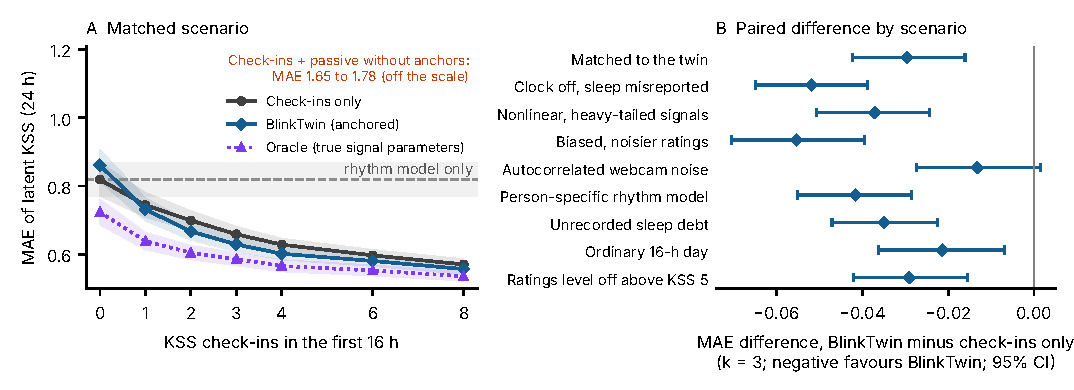
\includegraphics[width=\linewidth]{../results/fig_sim_mae.pdf}
  \caption{Simulation. (A) Mean absolute error of the latent KSS estimate over 24~h against the number of check-ins in the first 16~h, with 95\% bootstrap intervals (300 test participants). Horizontal lines: rhythm model only, and passive signals only. (B) Choice of the webcam noise inflation $\kappa$ on the separate tuning cohort (120 participants, three check-ins); ``off'' is the twin without the webcam.}
  \label{fig:sim}
\end{figure}
